\chapter{Evaluation}\label{ch:evaluation}

\section{Solved Problems}
The three main problems with existing smart homes, as outlined in Chapter~\ref{ch:lit_review}, are a constant requirement for internet access, interoperability between smart devices and systems, and the lack of true intelligence.
The goal of this thesis was to attempt to tackle some of these challenges.
By utilising local AI models for pose estimation and speech recognition, as well as using Home Assistant as the platform to control the devices in the home, this solves the issue as all computation is done on the local network, eliminating the need for an internet connection.
The system is still accessible from outside the home over the internet, but in the case that the network drops its connection, users within the house do not lose their ability to control their devices.
Using Home Assistant also solves the interoperability issue.
As an open source home automation platform, devices from previously incompatible communication standards can all be brought together and controlled under one system, whether they are compatible with Google, Apple or Amazon's platforms or if they use Bluetooth, Wi-Fi, Z-Wave, Zigbee or another proprietary standard.
Tackling the issue of true intelligence to the extent that was describe in the literature review, by utilising AI to predict user behaviour and patterns, was outside the scope of this thesis.
However, using AI for pose estimation and speech recognition does provide an added layer of quasi-intelligence to improve the landscape of the smart home industry.

One of the key rules that should be considered when developing any smart home or smart device is that functionality should always be added to, and never replaced.
A smart light that is no-longer controllable from the wall switch due to it's new smart features is not an improvement on the old system.
Technology is not perfect and fails every day.
If the smart features fail to work then the house is left completely inoperable.
In the deployment of this thesis, all devices had functionality added, and did not interrupt existing operation.
The light bulbs were still controllable by a physical switch, and in addition they had a new remote to control them, they could be controlled through the home assistant app or website and finally by voice commands and gestures.
The IR emitter allowed the television (TV) to be controlled by voice and gestures but the original TV remote was still available for regular use.

There were also some problems that had not been addressed in the existing literature that were solved in this thesis.
Hasnain et al. used YOLO for person detection but did not utilise the pose estimation capabilities, and additionally the automations they implemented were primitive, only allowing an on and off state of an LED~\cite{Hasn19}.
This thesis uses pose estimation for more advanced gesture detection and is capable of controlling devices with many more states than just on and off.
The TV can be controlled to turn it on and off, turn the volume up and down, and fast-forward and rewind the content being viewed.
The lights could also be controlled to toggle their power and change their brightness up and down.
Krumm et al. had employed a similar system, however were limited to 3.5Hz refresh rate of their cameras, which in this thesis has been increased to 30Hz~\cite{Krum00}.

Aluru et al. and Rani et al. both implemented voice control systems for the home through mobile apps.
However, as outlined in the literature review, this limits the convenience gained by requiring users to have their phone with them at all times to control devices as there was no stationary microphones throughout the home~\cite{Alur21,Rani17}.
Utilising the microphone of the computer used to run the software required, or another microphone plugged into it, means that the system is always ready and listening for commands.
Dutt et al. faced the challenge of only having a total 15 possible voice commands that occupants of the home could use to control their devices~\cite{Dutt20}.
This is not very user friendly and does not allow for a modular system with room to expand as more devices are added to the home.
With the web app implemented in this thesis, users are able to add their own commands and devices as they see fit. 
Finally, Ganji et al. had the most advanced system implemented of those covered in Chapter~\ref{ch:lit_review}, with more advanced gesture detection and device control.
However, due to the complicated nature of their implementation, it is still not a very accessible system for end users.
Devices and gestures in theory could be added to the system, but this would require significant technical knowledge and reprogramming the software to accommodate any new devices.
Utilising Home Assistant as the platform for the smart devices allows users to simply add new devices to the system themselves and modify which gesture and voice command combos control which devices.
Additionally, with the web app that was developed, users are able to add to and customise their list of allowed voice commands and devices.
This added level of flexibility makes it far more appealling for a real world deployment.

\section{System Evalutation}
After development was completed, three users were chosen to test the reliability of the system as show in Figure~\ref{fig:user1_testing} and Figure~\ref{fig:user2_testing}.
Each was given a script of 13 commands to read from, and were given the option to add their own words to the commands if they saw fit and attempt other related commands.

\begin{itemize}
    \item Turn on that light (With no gesture)
    \item Turn on that light
    \item Turn off that light
    \item Turn up that light
    \item Turn down that light
    \item Toggle that light
    \item Turn on all/every light(s)
    \item Turn on that TV
    \item Turn off that TV
    \item Turn up that TV
    \item Turn down that TV
    \item Fast forward that TV
    \item Rewind that TV
\end{itemize}

\begin{figure}[!htb]
    \caption{User 1 Testing}
    \centering
    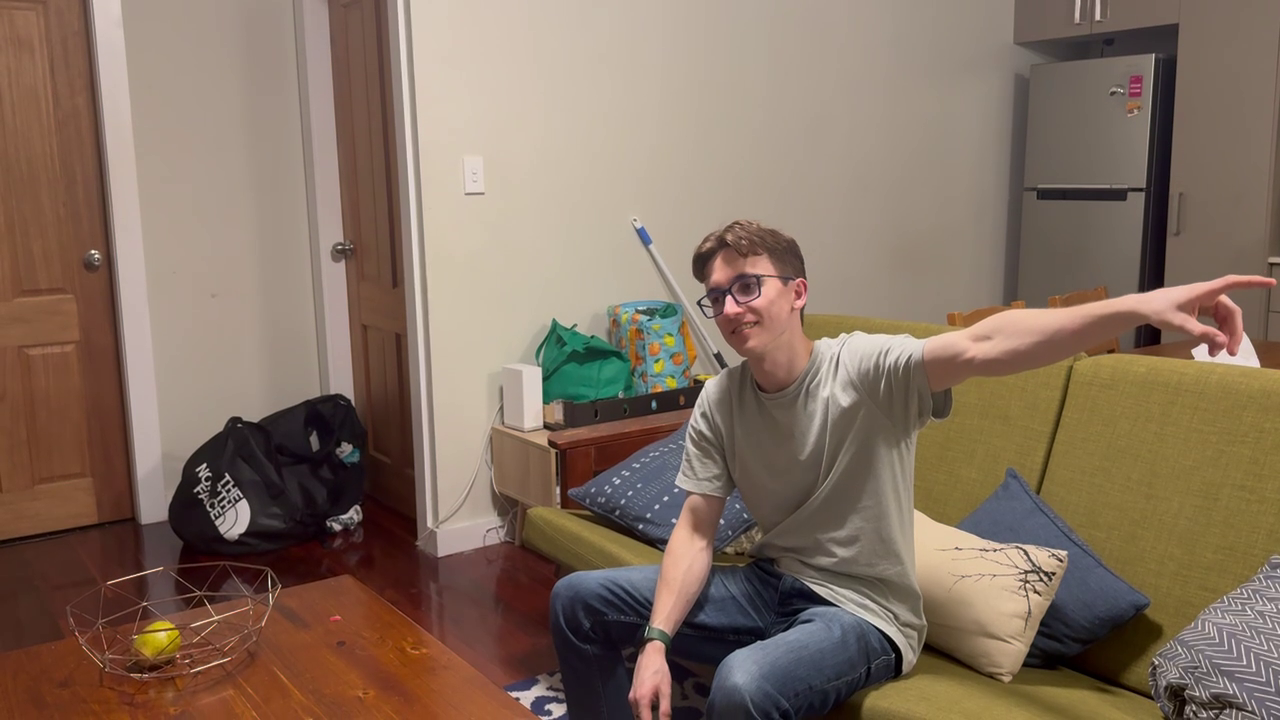
\includegraphics[width=0.6\textwidth]{User 1 Testing.png}
    \label{fig:user1_testing}
\end{figure}

\begin{figure}[!htb]
    \caption{User 2 Testing}
    \centering
    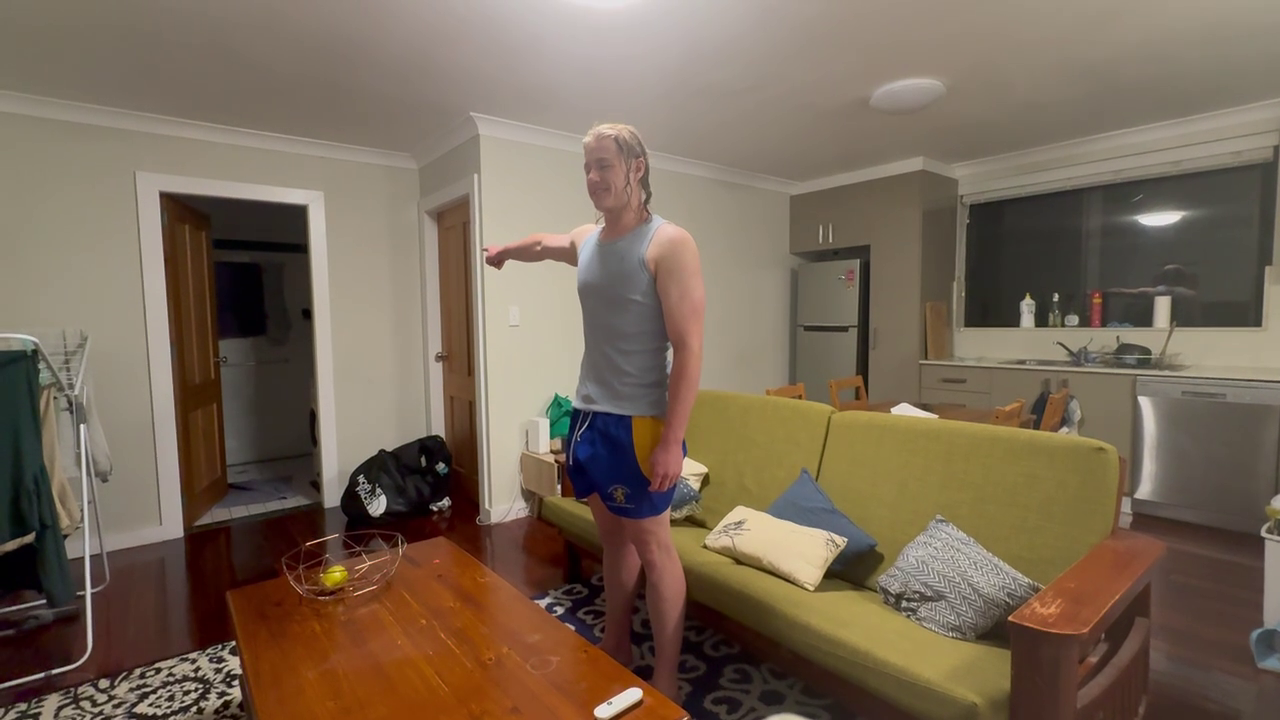
\includegraphics[width=0.6\textwidth]{User 2 Testing.png}
    \label{fig:user2_testing}
\end{figure}

\subsection{Quantitative Analysis}
Following these tests, the results were as shown in Table~\ref{tab:user_test_results}

\begin{table}[h!]
    \centering
    \begin{tabular}{|l|c|c|c|}
        \hline
        Result & User 1 & User 2 & User 3\\ \hline
        True Positive & 12 & 13 & 19 \\ \hline
        False Positive & 0 & 0 & 0 \\ \hline
        False Negative (Speech) & 5 & 7 & 7 \\ \hline
        False Negative (Gesture) & 0 & 0 & 2 \\ \hline
        Success (\%) & 71\% & 65\% & 68\% \\ \hline
    \end{tabular}
    \caption{User Testing Results}
    \label{tab:user_test_results}
\end{table}

In all cases, commands given with no gesture were correctly identified and the user was notified.
Additionally, on only two occasions was there a false negative result due to a gesture being misidentified.
Both of these were with user 3 and likely due to the fact that she was wearing a very loose jumper causing YOLO to select the incorrect location for the elbow as shown in Figure~\ref{fig:user3_testing}.
It could also possibly have been correctly selected by YOLO, but when the depth data at this coordinate was calculated, the loose fabric caused a smaller depth to be read.
There was also never any false positive results, meaning the system will never trigger a device automation without explicit input from the user.
Overall, the success rate was an average of 68\%, almost entirely due to verbal commands being misinterpreted and commands took approximately two to three seconds from the end of the sentence to the device being triggered.

\begin{figure}[!htb]
    \caption{User 3 Testing}
    \centering
    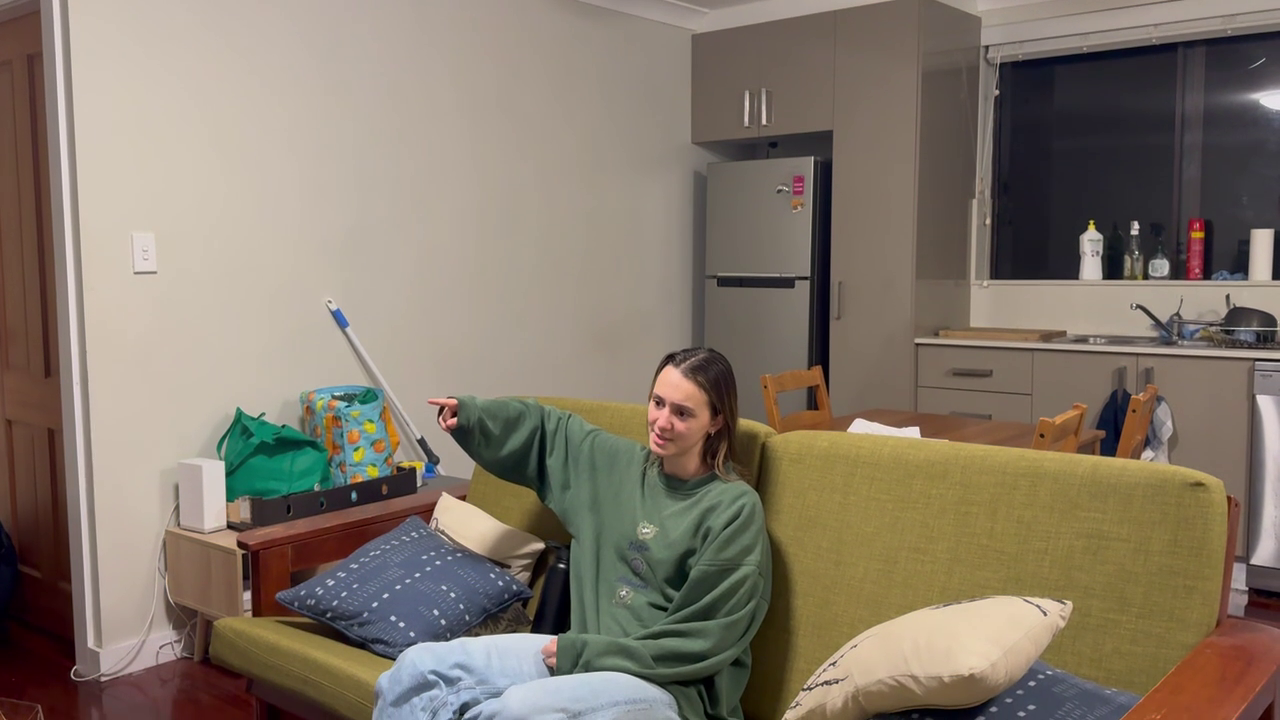
\includegraphics[width=0.6\textwidth]{User 3 Testing.png}
    \label{fig:user3_testing}
\end{figure}

OpenAI's Whisper STT model was explored for interpreting voice commands, however it does not support streaming to the model directly, meaning that in order to get it to work, chunks of audio had to be sent in five second snippets.
This causes a few problems, most notably that a command can be cut off mid sentence.
To solve this, the audio was sent in rolling 10 second clips every 5 seconds to maintain a full sentence.
The drawback with this is that it creates a significant delay in processing the commands making the system significantly slower.
Additionally, the timings with the Whisper model were far less consistent, meaning that aligning the timings with the keyword ``that'' when gesturing became an impossible task as it was non-deterministic.
Despite Whisper having much more accurate and consistent interpretations, because of these reasons it was unfeasible for use in this project.

In addition to the three users testing the system under standardised conditions, there were tests conducted under varying conditions with different types of background noise.
The three tests were with background talking, with background music with lyrics, and with background music without lyrics.

\begin{table}[h!]
    \centering
    \begin{tabular}{|l|c|c|c|}
        \hline
        Result & Background Talking & \makecell{Background Music \\ (with Lyrics)} & \makecell{Background Music \\ (Instrumental Only)} \\ \hline
        True Positive & 1 & 1 & 13 \\ \hline
        False Positive & 0 & 0 & 0 \\ \hline
        False Negative (Speech) & 12 & 15 & 7 \\ \hline
        False Negative (Gesture) & 0 & 0 & 0 \\ \hline
        Success (\%) & 8\% & 6\% & 65\% \\ \hline
    \end{tabular}
    \caption{User Testing Results}
    \label{tab:background_test_results}
\end{table}

With any amount of words being spoken in the background, whether it is conversation or lyrics in a song, even at a low volume, the accuracy of the model drops significantly to 8\% and 6\% respectively.
With instrumental only music playing in the background the accuracy of the model drops only marginally to 65\%.
With an approximate 90\% drop in accuracy, this solution is not suitable for use in an environment where there will be constant conversation, unless users are in a controlled environment and can pause discussions in order to trigger their commands.
In an environment with gentle music only a 5\% drop is recorded in preliminary testing and would be appropriate for deployment.

\subsection{Qualitative Analysis}
Users were surveyed after their testing, and the responses were relatively consistent.
All users considered that this system would overall provide an increase in convenience if it had been a little more polished.
When it worked, it was responsive and felt like a step towards a more advanced intelligent home environment.
However, the accuracy of the STT model was a big enough drawback that most would not want this in their homes yet.
With time for technology to improve and a better STT model operating this could be a promising prospect.

In environments with background speech, the system also experienced a significant slow down in processing speed of the STT model.
This created large delays in transcription, even once the speaking had stopped, until it had time to catch back up to itself during periods of quiet.
This could affect its use in busy homes if commands are not registered in time after long periods of high volume conversation.